\documentclass{article}
\usepackage{geometry}
\usepackage{graphicx}
\usepackage{float}
\usepackage{titlesec}
\geometry{a4paper, left=2cm, right=2cm, top=2cm, bottom=2cm}
\titleformat{\section}{\normalfont\fontsize{14}{15}\bfseries}{\thesection}{1em}{}
\usepackage{hyperref}
\usepackage{ctex}
\usepackage{caption}
\usepackage{subcaption}
\usepackage{listings}
\usepackage{xcolor}

% 设置代码样式
\lstdefinestyle{Style}{
    language=python, % 设置代码语言
    basicstyle=\ttfamily\small, % 设置字体样式和大小
    keywordstyle=\color{blue}, % 关键字颜色
    commentstyle=\color{green!40!black}, % 注释颜色
    stringstyle=\color{purple}, % 字符串颜色
    numbers=left, % 行号显示在左侧
    numberstyle=\tiny\color{gray}, % 行号样式
    stepnumber=1, % 行号逐行显示
    numbersep=8pt, % 行号与代码的距离
    showspaces=false, % 是否显示空格
    showstringspaces=false, % 是否显示字符串中的空格
    showtabs=false, % 是否显示制表符
    tabsize=4, % 制表符的大小
    frame=single, % 边框类型,可以是 single, lines, none, ...
    frameround=tttt, % 边框角落样式,可以是 tttt, trbl, none, ...
    backgroundcolor=\color{white}, % 背景颜色
    breaklines=true, % 自动断行
    breakatwhitespace=true, % 在空格处断行
    captionpos=b, % 代码块标题位置(b 表示底部)
    extendedchars=true, % 支持特殊字符
    morekeywords={val, var, def, import}, % 添加额外的关键字
    inputencoding=utf8, % 输入编码,适用于包含非 ASCII 字符的代码
}

\begin{document}
\title{新闻类别分类}
\author{211250109 赵政杰}
\date{\today}
\maketitle

\section{数据集描述}
通过analysis.py对数据集进行分析,结果如下:\par
Number of Samples: 208908\par
Number of Features: 6\par
同时分别生成了类别分布的柱状图、饼状图
\begin{figure}[H]
    \centering
    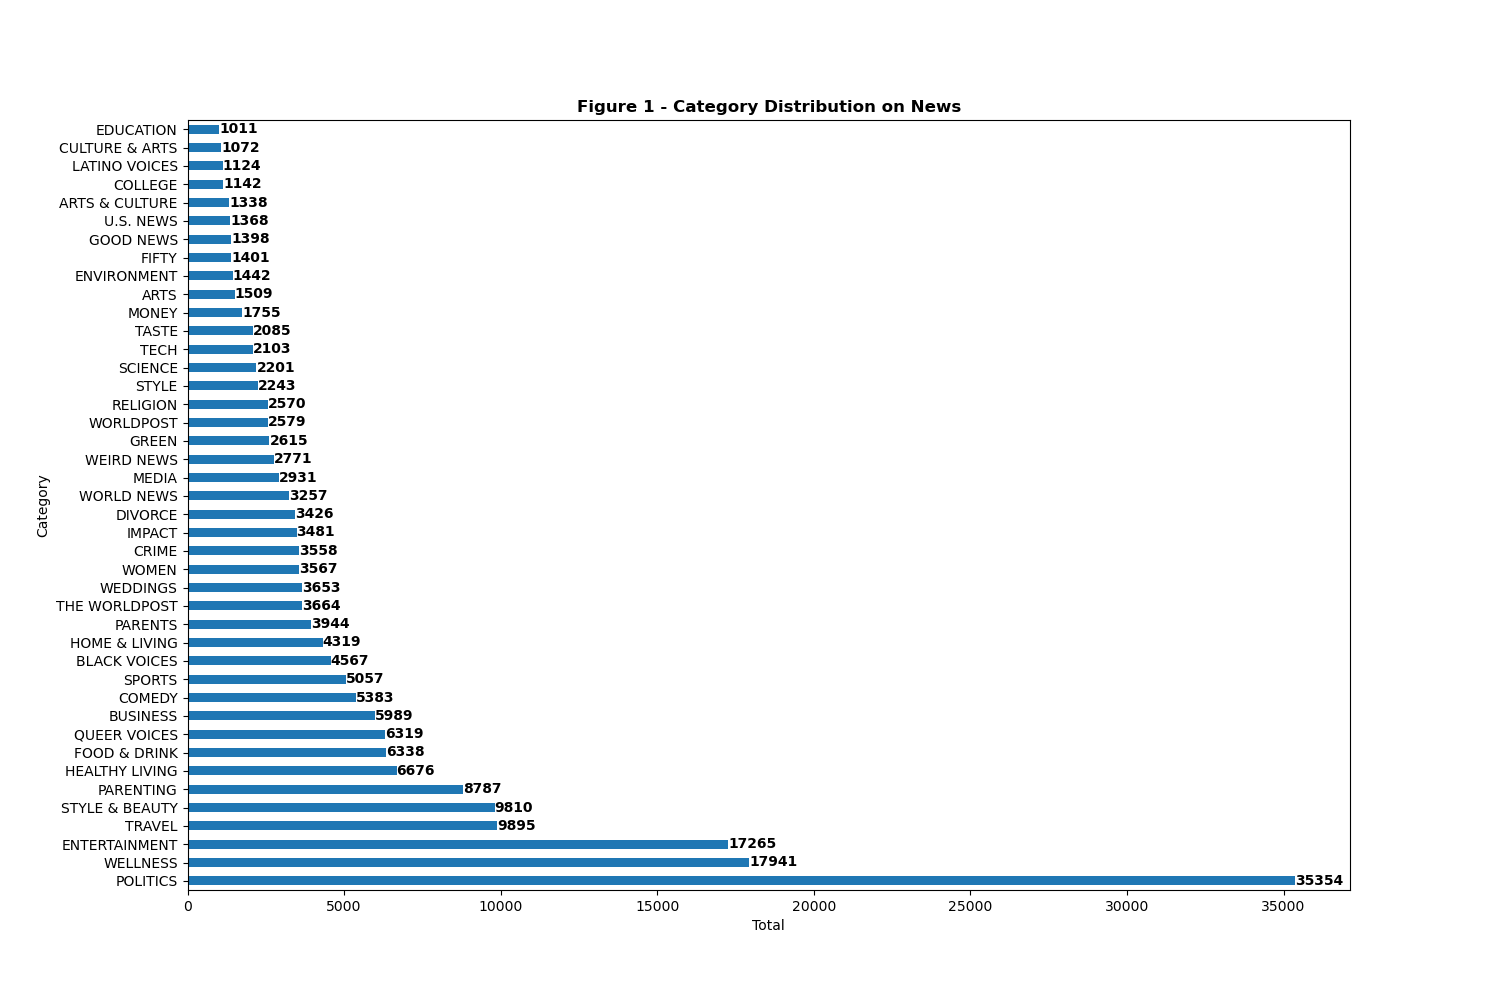
\includegraphics[width=0.5\textwidth]{./pic/1.png}
    \caption{柱状图}
\end{figure}

\begin{figure}[H]
    \centering
    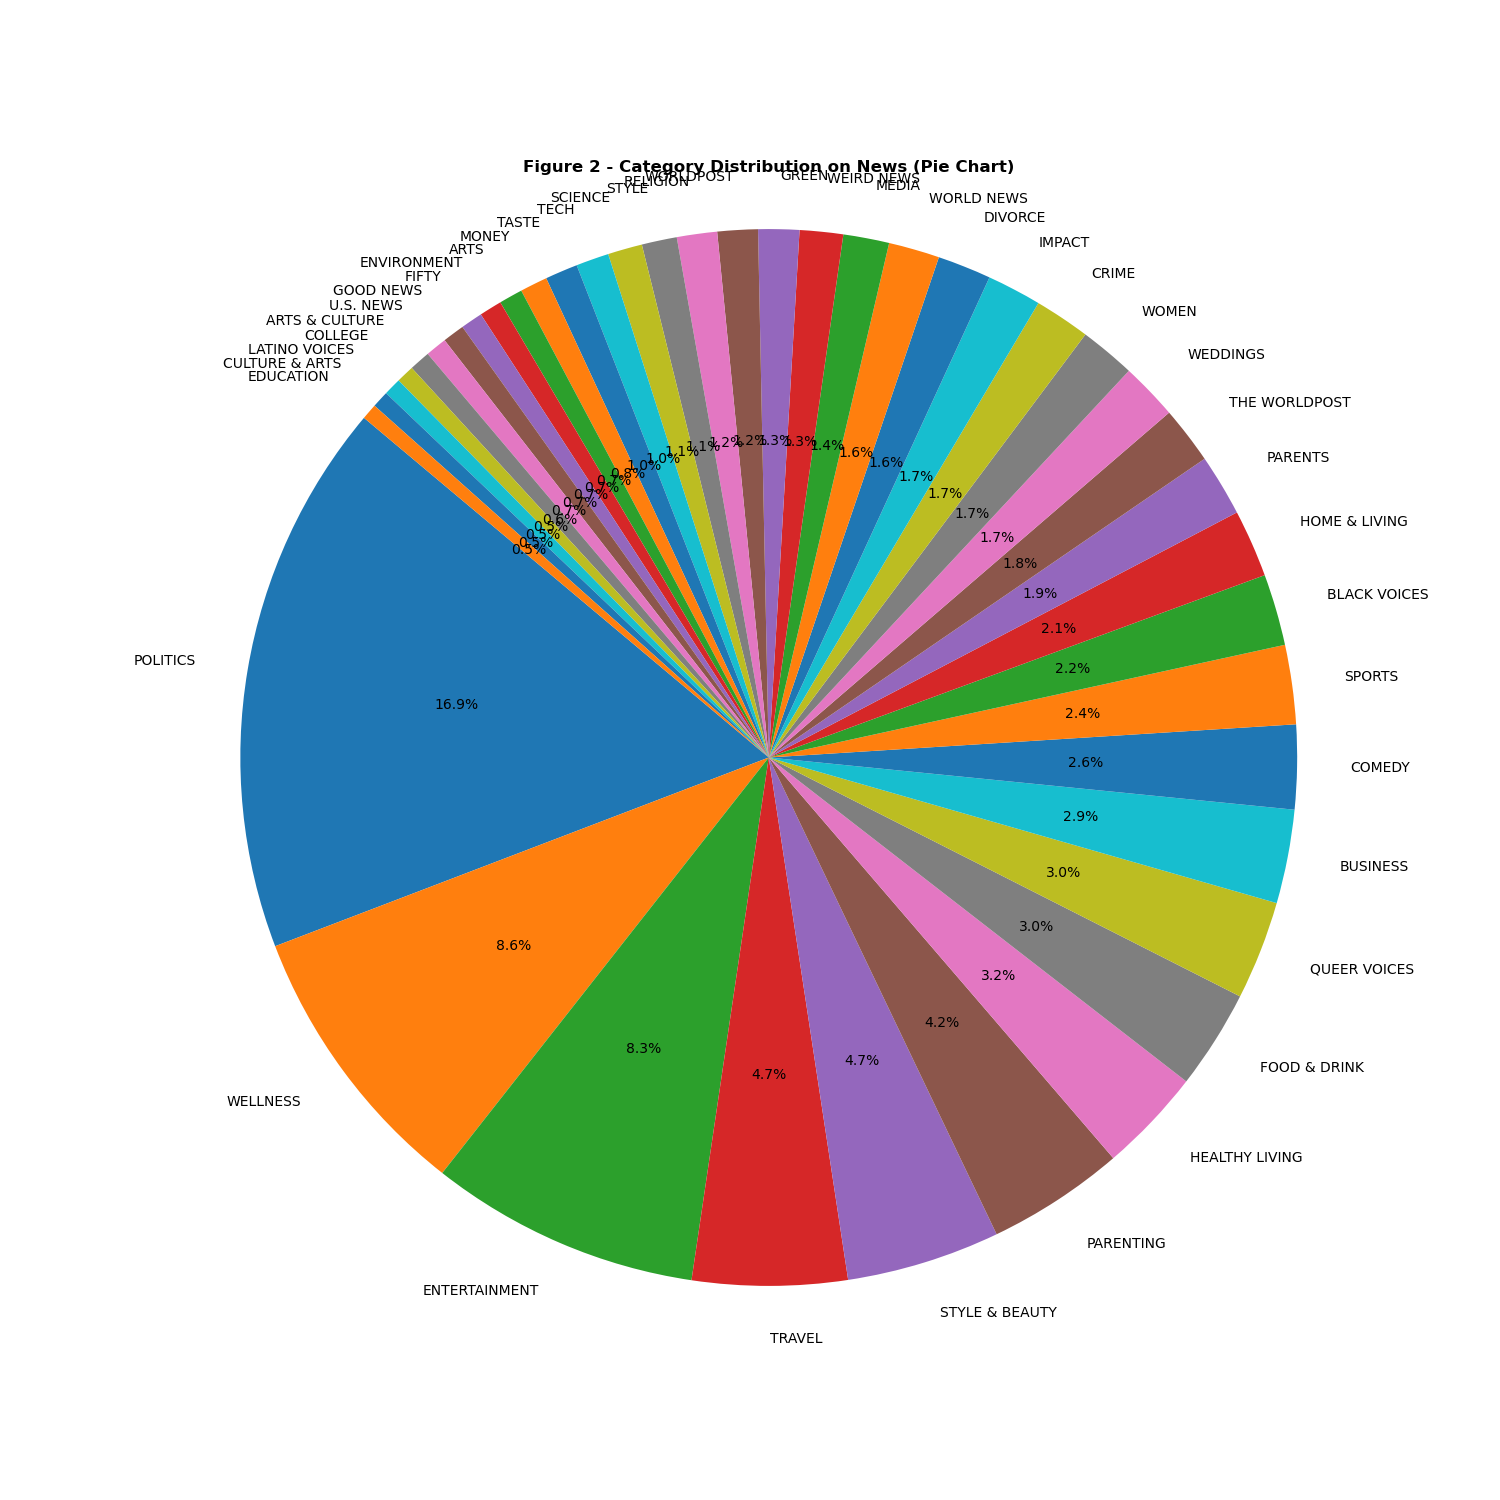
\includegraphics[width=0.5\textwidth]{./pic/2.png}
    \caption{饼状图}
\end{figure}
生成short\_description列中词语的词云图,如下
\begin{figure}[H]
    \centering
    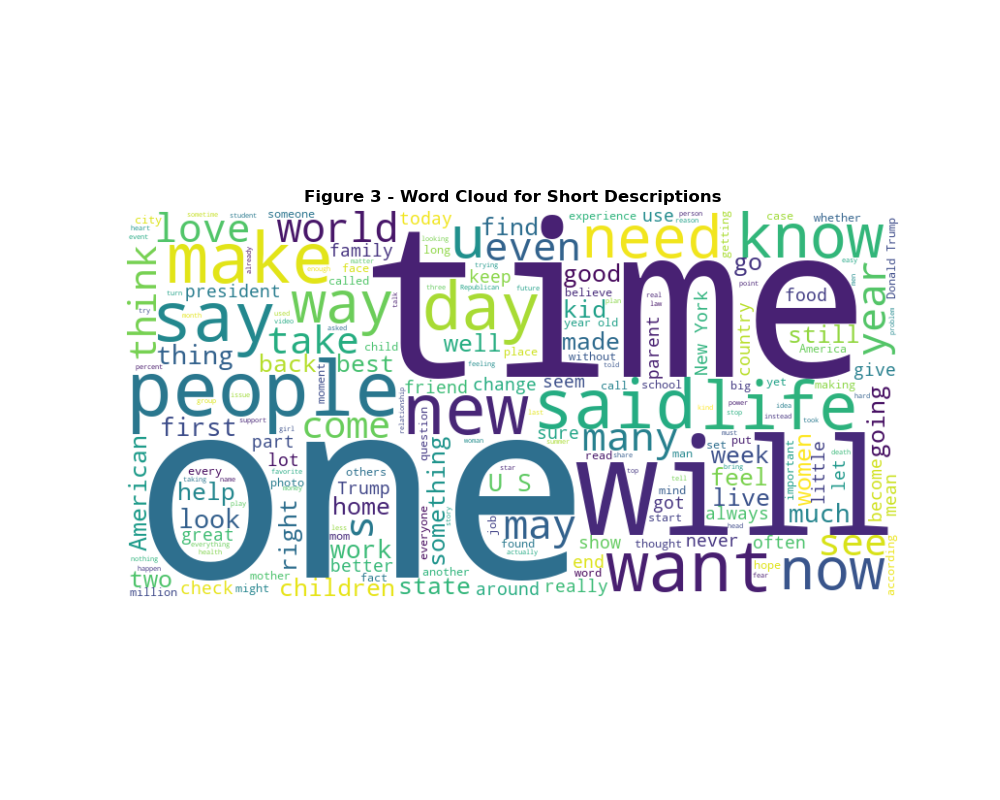
\includegraphics[width=0.7\textwidth]{./pic/3.png}
    \caption{词云图}
\end{figure}

\section{数据处理}
使用pandas库读取json文件,并将其存储在 Pandas DataFrame 中。\par
将\textbf{作者、新闻标题、link和简短描述}合并为一个文本列,并将类别作为标签列构建新的 DataFrame。\par
定义数据集类TextClassificationDataset,用来将数据集转化为相应的张量\par
实现代码如下:
\begin{lstlisting}[style=Style]
# TextClassificationDataset类定义
class TextClassificationDataset(Dataset):

    def __init__(self,
                 texts: List[str],
                 labels: List[str] = None,
                 label_dict: Mapping[str, int] = None,
                 max_seq_length: int = 512,
                 model_name: str = 'distilbert-base-uncased'):

        self.texts = texts
        self.labels = labels
        self.label_dict = label_dict
        self.max_seq_length = max_seq_length

        if self.label_dict is None and labels is not None:
            self.label_dict = dict(zip(sorted(set(labels)),
                                       range(len(set(labels)))))

        self.tokenizer = AutoTokenizer.from_pretrained(model_name)

        self.sep_vid = self.tokenizer.vocab["[SEP]"]
        self.cls_vid = self.tokenizer.vocab["[CLS]"]
        self.pad_vid = self.tokenizer.vocab["[PAD]"]

    def __len__(self):

        return len(self.texts)

    def __getitem__(self, index) -> Mapping[str, torch.Tensor]:

        x = self.texts[index]
        x_encoded = self.tokenizer.encode(
            x,
            add_special_tokens=True,
            max_length=self.max_seq_length,
            return_tensors="pt",
            truncation=True  # 明确启用截断
        ).squeeze(0)

        true_seq_length = x_encoded.size(0)
        pad_size = self.max_seq_length - true_seq_length
        pad_ids = torch.Tensor([self.pad_vid] * pad_size).long()
        x_tensor = torch.cat((x_encoded, pad_ids))

        mask = torch.ones_like(x_encoded, dtype=torch.int8)
        mask_pad = torch.zeros_like(pad_ids, dtype=torch.int8)
        mask = torch.cat((mask, mask_pad))

        output_dict = {
            "features": x_tensor,
            'attention_mask': mask
        }

        if self.labels is not None:
            y = self.labels[index]
            y_encoded = torch.Tensor(
                [self.label_dict.get(y, -1)]
            ).long().squeeze(0)
            output_dict["targets"] = y_encoded

        return output_dict


data_path = "./data"
data = pd.read_json(data_path+"/News_Category.json", lines=True)
text = pd.DataFrame({
    "text" : data.authors+" "+data.headline+" "+data.link+" "+data.short_description,
    "label" : data.category
})
train_dataset = TextClassificationDataset(
    texts=train['text'].values.tolist(),
    labels=train['label'].values.tolist(),
    label_dict=label_dict,
    max_seq_length=MAX_SEQ_LENGTH,
    model_name=MODEL_NAME
)
valid_dataset = TextClassificationDataset(
    texts=val['text'].values.tolist(),
    labels=val['label'].values.tolist(),
    label_dict=label_dict,
    max_seq_length=MAX_SEQ_LENGTH,
    model_name=MODEL_NAME
)
\end{lstlisting}
\section{分类模型选择及设计、训练、验证、测试}
实现在train.py文件、test.py文件和some\_classes.py文件中
\subsection*{3.1 模型选择与设计}
选择使用DistilBert模型进行分类。DistilBert是一种小型、快速和轻量级的Transformer模型,通过知识蒸馏BERT基础进行训练。\par
用于序列分类的DistilBERT模型定义如下:
\begin{lstlisting}[style=Style]
    class DistilBertForSequenceClassification(nn.Module):

    def __init__(self, pretrained_model_name: str, num_classes: int = None):

        super().__init__()

        config = AutoConfig.from_pretrained(
            pretrained_model_name, num_labels=num_classes)

        self.distilbert = AutoModel.from_pretrained(pretrained_model_name,
                                                    config=config)
        self.pre_classifier = nn.Linear(config.dim, config.dim)
        self.classifier = nn.Linear(config.dim, num_classes)
        self.dropout = nn.Dropout(config.seq_classif_dropout)

    def forward(self, features, attention_mask=None, head_mask=None):

        outputs = self.distilbert(input_ids=features, attention_mask=attention_mask, head_mask=head_mask)

        hidden_state = outputs[0]
        pooled_output = hidden_state[:, 0]
        pooled_output = self.pre_classifier(pooled_output)
        pooled_output = nn.ReLU()(pooled_output)
        pooled_output = self.dropout(pooled_output)
        logits = self.classifier(pooled_output)

        return logits
# 加载模型
model = DistilBertForSequenceClassification(pretrained_model_name=MODEL_NAME,
                                            num_classes=NUM_CLASSES)
\end{lstlisting}
\subsection*{3.2 训练与验证}
将数据集划分为80\%的训练集和20\%的验证集:
\begin{lstlisting}[style=Style]
train, val = train_test_split(text, test_size=0.20, random_state=SEED)
\end{lstlisting}
\hspace{2em}训练参数设置:
\begin{lstlisting}[style=Style]
MODEL_NAME = "distilbert-base-uncased"
NUM_EPOCHS = 3
BATCH_SIZE = 80
MAX_SEQ_LENGTH = 256
LEARN_RATE = 5e-5
SEED = 42
LOG_DIR = 'results'
\end{lstlisting}
\hspace{2em}训练与验证过程如代码所示:
\begin{lstlisting}[style=Style]
model = DistilBertForSequenceClassification(pretrained_model_name=MODEL_NAME,
                                            num_classes=NUM_CLASSES)
criterion = torch.nn.CrossEntropyLoss()
optimizer = torch.optim.Adam(model.parameters(), lr=LEARN_RATE)
scheduler = torch.optim.lr_scheduler.ReduceLROnPlateau(optimizer)

device = torch.device('cuda' if torch.cuda.is_available() else 'cpu')
model.to(device)
for epoch in range(NUM_EPOCHS):
    # Training loop
    model.train()
    total_loss = 0

    for batch_idx, batch in enumerate(train_val_loaders['train']):
        optimizer.zero_grad()

        features = batch['features'].to(device)
        attention_mask = batch['attention_mask'].to(device)
        targets = batch['targets'].to(device)

        outputs = model(features, attention_mask=attention_mask)
        loss = criterion(outputs, targets)
        total_loss += loss.item()

        loss.backward()
        optimizer.step()

        if batch_idx % 10 == 0:
        print(f"Epoch [{epoch + 1}/{NUM_EPOCHS}] "
              f"Batch [{batch_idx + 1}/{len(train_val_loaders['train'])}] "
              f"Loss: {loss.item()}")
        logging.info(f"Epoch [{epoch + 1}/{NUM_EPOCHS}] "
                     f"Batch [{batch_idx + 1}/{len(train_val_loaders['train'])}] "
                     f"Loss: {loss.item()}")

    average_loss = total_loss / len(train_val_loaders['train'])
    print(f"Epoch [{epoch + 1}/{NUM_EPOCHS}] "
          f"Average training loss: {average_loss}")
    logging.info(f"Epoch [{epoch + 1}/{NUM_EPOCHS}] "
                 f"Average training loss: {average_loss}")

    # Validation loop
    model.eval()
    val_loss = 0
    predicted_labels = []
    true_labels = []

    with torch.no_grad():
        for val_batch in train_val_loaders['valid']:
            features = val_batch['features'].to(device)
            attention_mask = val_batch['attention_mask'].to(device)
            targets = val_batch['targets'].to(device)

            outputs = model(features, attention_mask=attention_mask)
            loss = criterion(outputs, targets)
            val_loss += loss.item()

            _, predicted = torch.max(outputs, 1)

            predicted_labels.extend(predicted.cpu().numpy())  # 预测的标签
            true_labels.extend(targets.cpu().numpy())  # 真实的标签

    average_val_loss = val_loss / len(train_val_loaders['valid'])
    acc = accuracy_score(true_labels, predicted_labels)  # 计算准确率
    precision = precision_score(true_labels, predicted_labels, average='macro')  # 计算精确度
    f1 = f1_score(true_labels, predicted_labels, average='macro')  # 计算F1 Score
    print(f"Epoch [{epoch + 1}/{NUM_EPOCHS}] "
          f"Test Accuracy: {acc}, Test Precision: {precision}, Test F1 Score: {f1}")
    logging.info(f"Epoch [{epoch + 1}/{NUM_EPOCHS}] "
                 f"Test Accuracy: {acc}, Test Precision: {precision}, Test F1 Score: {f1}")

    # 根据验证损失调整学习率
    scheduler.step(average_val_loss)
    # 保存训练好的模型
    torch.save(model.state_dict(), f'results1/trained_model_epoch_{epoch + 1}.pth')
\end{lstlisting}
\subsection*{3.3 测试}
加载训练好的模型文件,在数据集上进行测试,实现如下:
\begin{lstlisting}[style=Style]
# 加载训练好的模型
loaded_model = DistilBertForSequenceClassification(pretrained_model_name=MODEL_NAME,
                                                   num_classes=NUM_CLASSES)
loaded_model.load_state_dict(torch.load('results/trained_model_epoch_2.pth')) # 替换成你想要加载的模型文件名
# 设置模型为评估模式

device = torch.device('cuda' if torch.cuda.is_available() else 'cpu')
loaded_model.to(device)

def cal_acc_test():
    test_loader = DataLoader(test_dataset, batch_size=100, shuffle=False)
    predicted_labels = []
    true_labels = []

    with torch.no_grad():
        for batch in test_loader:
            features = batch['features'].to(device)
            attention_mask = batch['attention_mask'].to(device)
            targets = batch['targets'].to(device)

            outputs = loaded_model(features, attention_mask=attention_mask)
            _, predicted = torch.max(outputs, 1)

            predicted_labels.extend(predicted.cpu().numpy())  # 预测的标签
            true_labels.extend(targets.cpu().numpy())  # 真实的标签

        acc = accuracy_score(true_labels, predicted_labels)  # 计算准确率
        precision = precision_score(true_labels, predicted_labels, zero_division=1, average='macro')  # 计算精确度
        f1 = f1_score(true_labels, predicted_labels, average='macro')  # 计算F1 Score
        print(f"Test Accuracy: {acc}, Test Precision: {precision}, Test F1 Score: {f1}")

if __name__ == "__main__":
    print_classifications_test()
\end{lstlisting}
\subsection*{3.4 训练结果}
参见模型链接中的log文件

\end{document}